
\BiChapter{相关理论}{TODO}
\label{chap:part2}

\BiSection{光场技术基本理论}{TODO}

光场的概念由A.Gershun~\cite{gershun1939light}教授提出,是空间中光线集合的完备表示,采集并显示光场就能在视觉上重现真实世界。
1991年,MIT的Edward H.Adelson教授和James R.Bergen\cite{adelson1991plenoptic}教授指出人眼对光线的视觉感知可以认为是沿着单一函数的一个或多个方向的局部变化,描述了光照射到观察面的信息结构。
一旦定义了这个函数,各种潜在的视觉属性(如运动、颜色和方向)的测量就能够自动分离出来。
这个函数被称为全光函数,表示为:
%$$$$
\begin{equation}
	L(x,y,z,\theta,\varphi,\lambda,t)
\end{equation}\par
其中$(x,y,z)$为发光物体的空间位置,$(\theta,\varphi)$分别表示传播光线入射的垂直角度和水平角度,$\lambda$表示传播光线的波长,发光物体所发射的光线信息随时时间$t$的推移而变化。


然而,这种能够记录空间中光线信息的七维全光函数过于复杂、数据量大,难以记录和存储,在实际计算中并未得到应用。
需要对其进行简化处理。
McMillan等~\cite{mcmillan2023plenoptic}在七维全光函数的基础上提出了简化波长和时间的更为方便的五维光场模型。
通过记录红、绿、蓝三原色来简化波长$\lambda$,通过记录不同帧来简化时间$t$。
如果不考虑光线在空间传播过程中的衰减,记录光场信息的五维模型还可以进一步简化成四参数光场函数。
Levoy等~\cite{levoy2023light}忽略掉传播距离维度$z$得到四维光场模型,
发展出了适用于光学系统的光场双平面参数特征。
\begin{figure}[!ht]
	\centering
	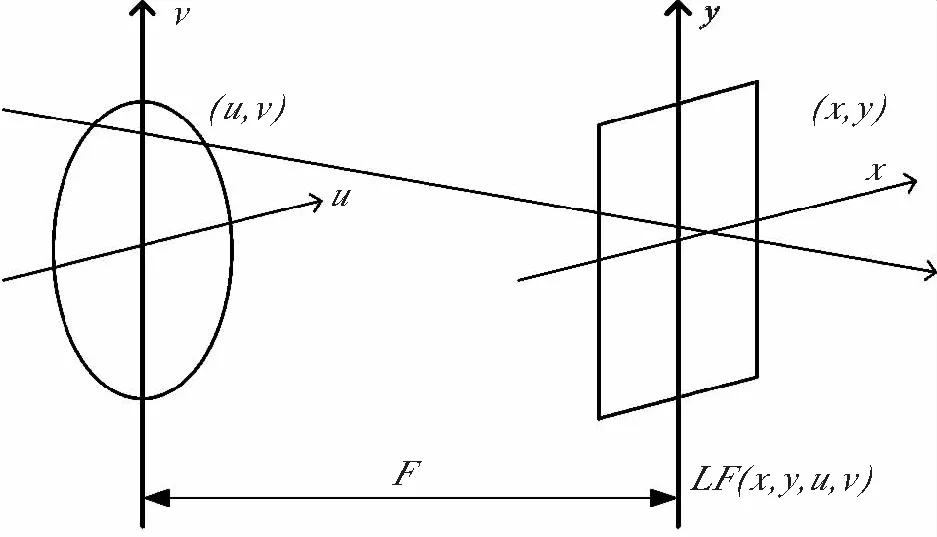
\includegraphics[width=0.78\linewidth]{figures/chapter2/double-plane2}
	\bicaption{光场双平面四参数模型}{Light field biplane four-parameter model}  
	\label{chapter2_fig1:double_plane}
\end{figure}
光线在空间传播中,因传播距离而造成的信息损耗微乎其微,光场模型完全可以以简化的四参数模型表示。




% \emph{et~al.}~
%光场是计算机科学领域的学者定义的“Light Field”,是指除了包含原图像矩阵中的空间坐标$(x,y)$和强度$I$外,还有光线入射的角度信息$(\theta,\varphi)$。
%光在传播过程中的各种潜在的视觉属性(如运动、颜色和方向)。


\BiSubsection{光场成像原理}{TODO}
\BiSubsection{光场数据可视化}{TODO}

\BiSection{光场显著性目标检测相关理论}{TODO}

\BiSubsection{基于多视角图像的显著性目标检测原理}{TODO}
\BiSubsection{基于焦点堆栈的显著性目标检测原理}{TODO}
\BiSubsection{显著性目标检测性能评估指标}{TODO}


\BiSection{本章小节}{TODO}

本章首先阐述了光场技术的基本理论,介绍了光场的成像原理以及数据可视化形式;
然后介绍了光场显著性目标检测的相关理论,分别描述了基于多视角图像的显著性目标检测、
基于焦点堆栈的显著性目标检测方法的实现原理,
并引入了显著性目标检测中常用的几种性能评价指标。